%%%%%%%%%%%%%%%%%%%%%%%%%%%%%%%%%%%%%%%%%%%%%%%%%%

%% % Preamble %%%

\documentclass[aspectratio=169]{beamer}

 %redefined colors for beamer 
\definecolor{beamer@nihblue}{RGB}{0,82,136} 
\definecolor{beamer@nihgrey}{RGB}{90,91,93} 
\definecolor{beamer@uiucgray}{RGB}{210,210,210} % gray for frame title background
\definecolor{beamer@uiucgray2}{RGB}{244,244,244} 

\usetheme{AnnArbor}
\setbeamercolor{frametitle}{fg=beamer@nihgrey,bg=beamer@uiucgray}
\usecolortheme{wolverine} 
  

 \setbeamercolor{normal text}{fg=black} 
 \setbeamercolor{title}{fg=white,bg=beamer@nihblue} 
 \setbeamercolor{item projected}{fg=white,bg=beamer@nihgrey} 
  
 % Boxes 
 \setbeamercolor{block title}{fg=beamer@nihgrey,bg=beamer@nihblue} 
 \setbeamercolor{block body}{fg=blue,bg=beamer@nihgrey} 
 \setbeamercolor{title in head/foot}{fg=beamer@uiucgray,bg=beamer@uiucgray} % ensures the middle portion between author name colored bar (blue) and page number (colored nihgrey color bar) is the uiuc gray option
 \setbeamercolor{author in head/foot}{fg=white,bg=beamer@nihblue} 
 \setbeamercolor{institute in head/foot}{fg=white,bg=beamer@nihgrey} 
 \setbeamercolor{date in head/foot}{fg=white,bg=beamer@nihgrey} 
 \setbeamercolor{section in head/foot}{fg=white,bg=beamer@nihblue} 
 \setbeamercolor{subsection in head/foot}{fg=white,bg=beamer@nihgrey} 


%% Bullet styles and colors %%
\setbeamercolor{itemize item}{fg=beamer@nihgrey}
\setbeamercolor{itemize subitem}{fg=beamer@nihblue}
\setbeamercolor{itemize subsubitem}{fg=beamer@nihblue}
\setbeamertemplate{itemize item}{\tiny\raise1.25pt\hbox{\donotcoloroutermaths$\blacksquare$}}            % First level item
\setbeamertemplate{itemize subitem}{\tiny\raise1.25pt\hbox{\donotcoloroutermaths$\blacktriangleright$}}      % Second level item
\setbeamertemplate{itemize subsubitem}{\tiny\raise1.25pt\hbox{\donotcoloroutermaths$\blacktriangleright$}}   % Third level item


% logo for each slide to appear in bottom right hand corner (the paperwidth value controls horizontal % placement
\logo{
\includegraphics[scale=0.08]{images-logos/nih-logo.png}\hspace*{.02\paperwidth}}


% change table of contents bullet styles to circles instead of spheres (can also use `square` as well) % change subsections to numbered list and make the font size of subsections smaller
\setbeamertemplate{section in toc}[circle]
\setbeamertemplate{subsection in toc}[subsections numbered]
\setbeamerfont{subsection in toc}{size=\scriptsize}


%% add progress bar to footline %%
\addtobeamertemplate{headline}{%
  \leavevmode%
  \hbox{%
  \begin{beamercolorbox}[wd=\paperwidth,ht=2.25ex,dp=1ex,center]{section in head/foot}%
     \insertsectionnavigationhorizontal{\paperwidth}{}{}
  \end{beamercolorbox}}%

}



%% Citations/bibtex
\usepackage[style=numeric-comp,%
            autocite=footnote,%
             backend=bibtex8,%
             firstinits=true,%. %% abbreviates first name to just letters and not full first name
             ]{biblatex}
\addbibresource{01-apha-2023-slide-deck.bib}

% redefine command for foot cite-makes it smaller
\newrobustcmd*{\footlessfullcite}{\AtNextCite{\renewbibmacro{title}{}\renewbibmacro{in:}{}\renewbibmacro{urldate}{}}\footfullcite} %remove in:', title and urldate

\AtEveryCitekey{\clearfield{pages}}  %get rid of pages from footnote citation
\AtEveryCitekey{\clearfield{issn}} %get rid of issn from footnote citation
\AtEveryCitekey{\clearfield{volume}} %get rid of volume from footnote citation
\AtEveryCitekey{\clearfield{number}} %get rid of number from footnote citation
\AtEveryCitekey{\clearfield{eprint}} %get rid of eprint from footnote citation
\AtEveryCitekey{\clearfield{url}} %get rid of url from footnote citation
\AtEveryCitekey{\clearfield{month}} %get of month from footnote citation
\AtEveryCitekey{\clearlist{language}} %get rid of language from footnote citation (note \clearlist and note clearfield
\AtEveryCitekey{\clearlist{abstract}}  %get rid of abtract from footnote citation
\setbeamerfont{footnote}{size=\tiny} %make citations tiny in the footnote


% for graph/diagram of dietary patterns
\usepackage{tikz}
\usetikzlibrary{arrows} % for arrow types in tikz



% for resizing tables
\usepackage{adjustbox}

% for multiple rows in one cell
\usepackage{pbox}

% for smaller than \tiny font
\usepackage{graphicx}

% some more colors
\usepackage{xcolor}

% for colored boxes around text
\usepackage{tcolorbox}

% multiple columns for TOC
\usepackage{multicol}

%% for github icon
\usepackage{fontawesome}
%% End of Preamble %%

%% End of Preamble %%

%%%%%%%%%%%%%%%%%%%%%%%%%%%%%%%%%%%%%%%%%%%%%%%%%%


% % title page preamble %%
\title
[]{\Large County-level Food Insecurity and COVID-19 Mortality in the United States: A Spatial
	Analysis with R-INLA}

\author[Maino Vieytes CA]{Christian Maino Vieytes, PhD MS} % name in [ ] is what goes in  footline, the name in brackets is what goes on title page

%% Institute name and U of I workmark %%
%% Institute name and U of I workmark %%
\institute[]{\color{beamer@nihgrey}Laboratory of Epidemiology \& Population Sciences (LEPS) \\ % use [] to not have the institute name on the footline
\vspace{7px} % space between name for LEPS and NIA logo

\includegraphics[scale=0.065]{images-logos/nia-logo.svg.png} } % note that the insertion  of the U of I 

%  % workmark occurs within the \institute
\date[]{ November 13, 2023} % [] removes the date from the footline

%% end title page preamble %%





%% Start of Document %%
\begin{document}
	
%% custom/local formatting of title slide %%
{
	\setbeamertemplate{logo}{} % use of the preceding opening brace and this command removes logo % % from the title page
	
	% add U of I color banner to top of slide and remove  navigation bar
	\setbeamertemplate{headline}{  
		\begin{beamercolorbox}[ht=3ex,wd=1\textwidth]{section in head/foot}
		\end{beamercolorbox} %
		% redefine headline locally for title frame
		\begin{beamercolorbox}[ht=3ex,wd=1\textwidth]{block title}
		\end{beamercolorbox} 
		\begin{beamercolorbox}[ht=2ex,wd=1\textwidth]{white}
		\end{beamercolorbox} 
	}
	\begin{frame}
		\titlepage{}
	\end{frame}
}


\section{Introduction}
% introeduce racial disparities during pandemic
\subsection{Racial Disparities During the COVID-19 Pandemic}
\begin{frame}
	\centering
	\begin{figure}
	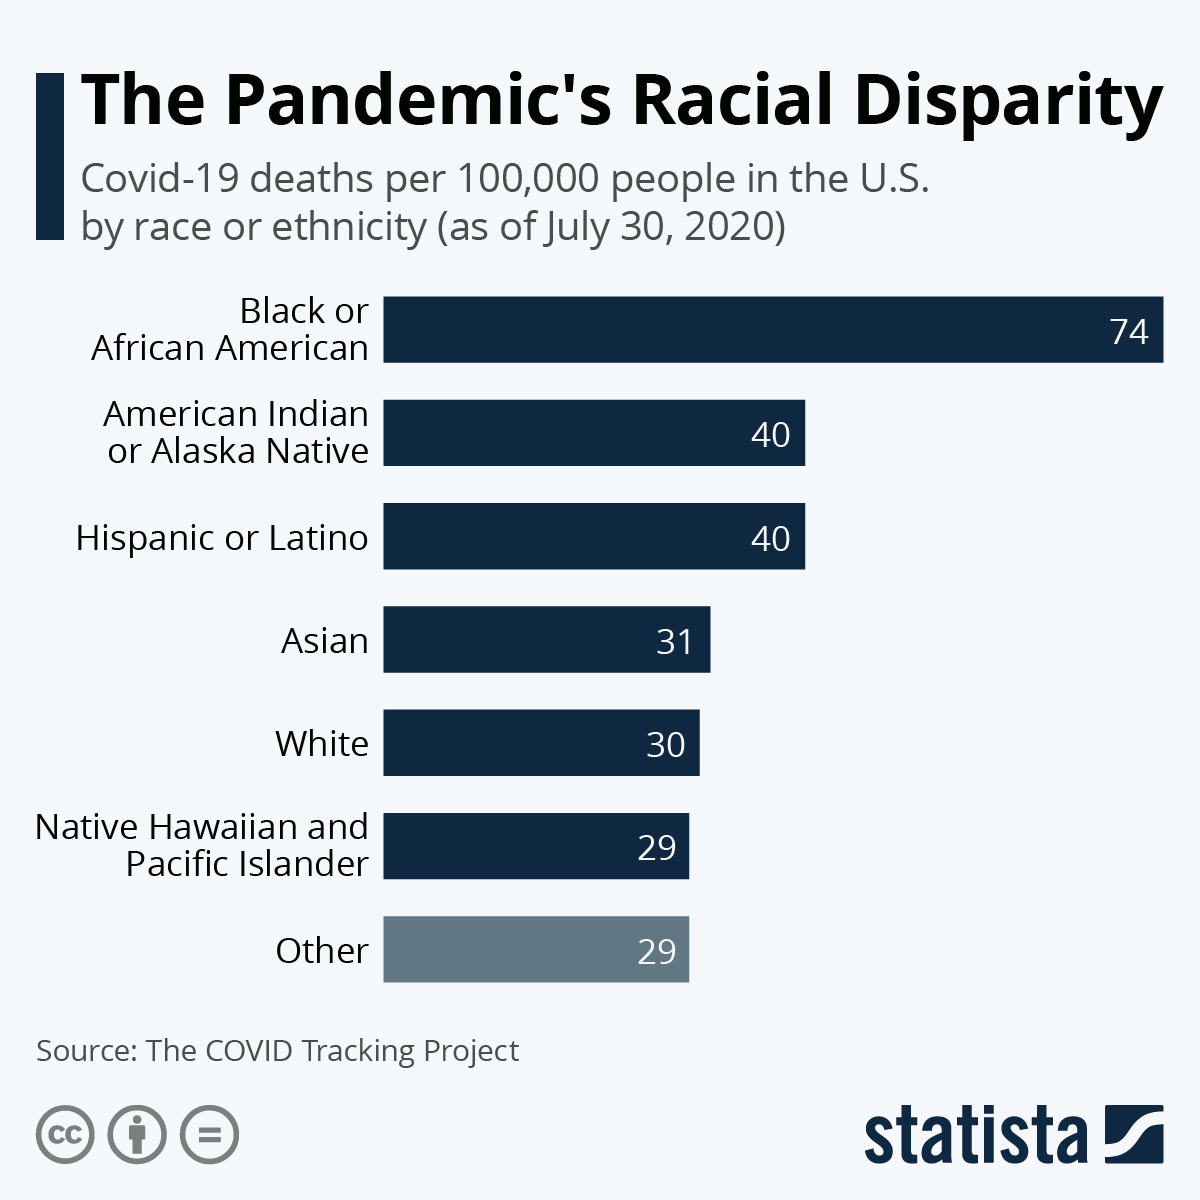
\includegraphics[scale=0.152]{images-logos/rac-disp.jpeg}\\
	
	\vspace{0.3cm}
	
	\tiny{Disparities in COVID-19 mortality during the early pandemic \footfullcite{niall_statista} }
		\end{figure}
\end{frame}

% define FI
\subsection{What is Food Insecurity?}
\begin{frame}
	\frametitle{Defining Food Insecurity}
	
	
	According to the United States Dept. of Agriculture (USDA) \textbf{food insecurity} (FI) is defined as: \textit{a lack of consistent  to enough food for every person in a household to live an active, healthy life.}
	
\end{frame}

\begin{frame}
	\frametitle{FI in the United States}
	\begin{itemize}
		\item 13.8 million FI households  across the U.S. (10.5\%) in 2020\footlessfullcite{coleman-jensen_household_2020}
		\begin{itemize}
			\item Low-income\footnote{Household income below 130\% of the poverty line}  households: 31.2\% prevalence in 2021\footlessfullcite{coleman-jensen_statistical_2022}
		\end{itemize}
		\item Racism and housing inequality
		\begin{itemize}
			\item Housing/redlining and supermarket redlining\footlessfullcite{shaker_redlining_2022}
		\end{itemize}       
		\item Government welfare programs mitigate FI \footlessfullcite{swann_household_2017}   
		 \begin{itemize}
			\item The Supplemental Nutrition Assistance Program (SNAP)
			\item Women, Infants, and Children (WIC)
			\item The National School Lunch Program
		\end{itemize}
	\end{itemize}
\end{frame}



%% FI and health outcomes

\begin{frame}
	\frametitle{FI and Health Outcomes}
	
	\begin{itemize}
		\item FI is associated with deleterious health outcomes\footlessfullcite{gundersen_food_2015}$^{,}$\footlessfullcite{seligman_hunger_2010}
		\begin{itemize}
			\item Hypertension
			\item Hyperlipidemia
			\item Depression and suicidal ideation
			\item Diabetes mellitus
			\item Iron deficiency anemia
		\end{itemize}
		
		\item Posited mechanisms
		\begin{itemize}
			\item Cortisol
			\item Diet quality, inflammation
			\item Competing demands and trade-offs
		\end{itemize}
	\end{itemize}
\end{frame}

  %hypotheses and rq
\subsection{Research Question and Hypothesis}

%hypotheses and rq
\begin{frame}
	
	\begin{center}
		\textbf{Research Question}: \textit{Is county-level food insecurity associated with COVID-19 mortality during the first 1.5 years of the COVID-19 pandemic?}\\
		
		\vspace{1.5cm}
		
		\textbf{Hypothesis}: We hypothesize that county-level food insecurity, given its association with other health outcomes, will adversely predict county-level COVID-19 deaths.
	\end{center}
\end{frame}

 \section{Methods}
 \subsection{Variables}
\begin{frame}
	\frametitle{Analysis Plan}
\begin{itemize}
	\item Variables
	\begin{itemize}
		\item \textit{Dependent variable}: \textbf{County-level COVID-19 death count}
		\begin{itemize}
			\item \textit{Source \#1}: John Hopkins University Coronavirus Resource Center (age-standardized via \textit{indirect standardization})
			\item \textit{Source \#2}: Provisional CDC restricted access case-level data (age-standardized via \textit{direct standardization})
			\item \textit{Time window}: 03/25/2020-12/25/2021
		\end{itemize}
		\vspace{0.2cm}
		\item \textit{Independent variable}: \textbf{County-level food insecurity prevalence (\%) (2020)} (\textit{source}: Feeding America's Map the Meal Gap)
		\vspace{0.2cm}
		\vspace{0.2cm}
	\end{itemize}
\end{itemize}
\end{frame}


\begin{frame}
	\frametitle{Covariates}
	\begin{minipage}{.52\textwidth}
		\hspace{-0.5cm}
		\centering
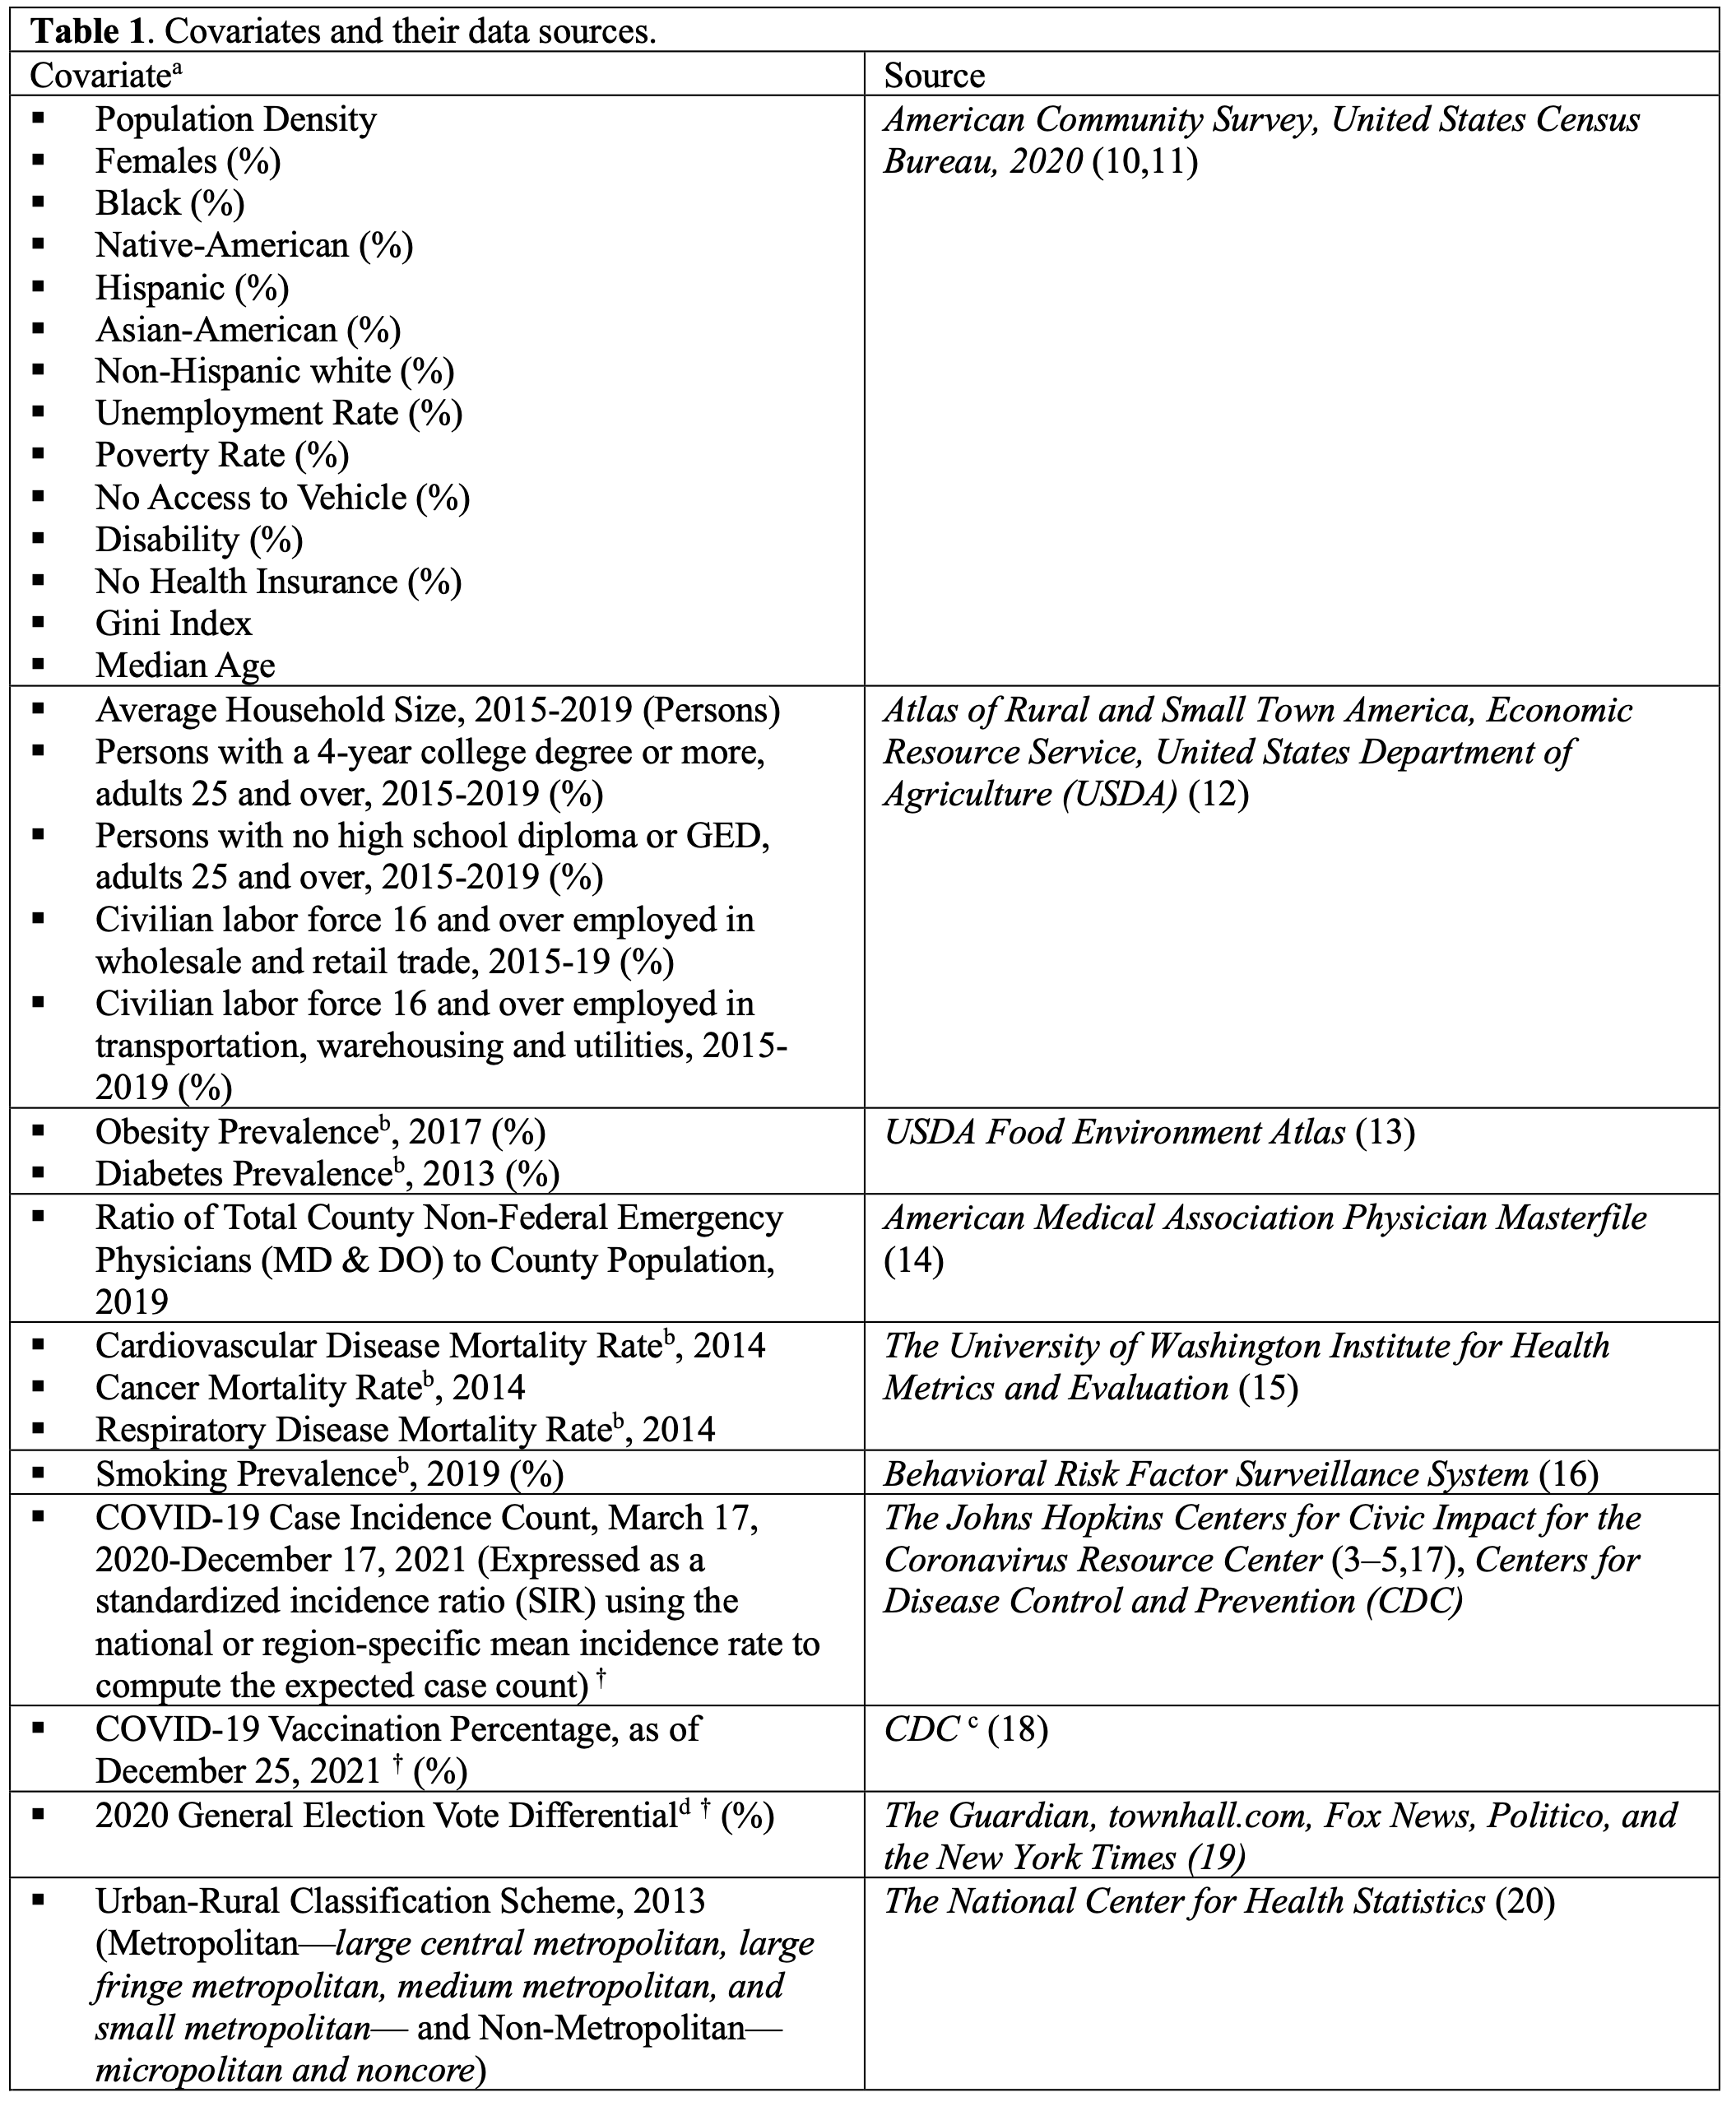
\includegraphics[scale=0.075]{images-logos/covariates-table.png}\\


	\end{minipage}% the '%' is important for putting the mini pages side by side and not stacked
	\begin{minipage}{.48\textwidth}

		\raggedleft
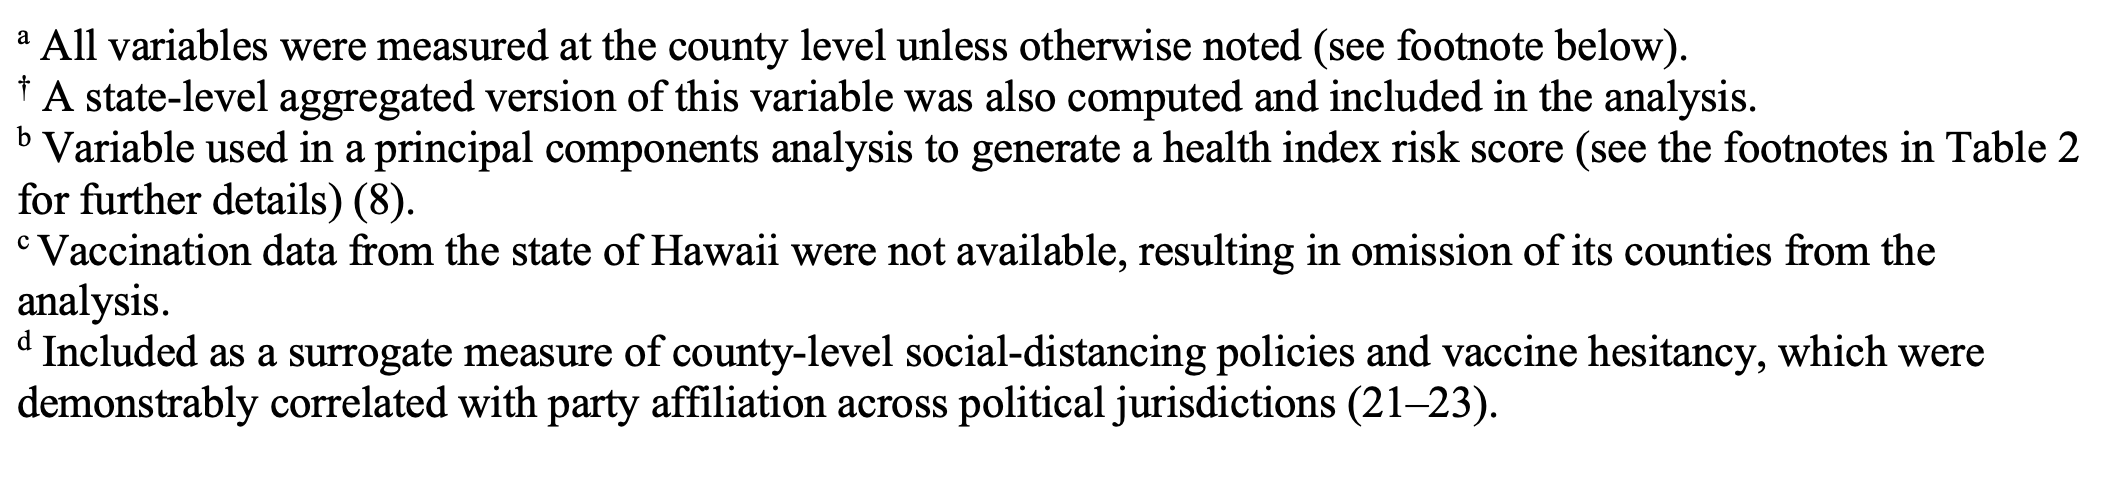
\includegraphics[scale=0.083]{images-logos/covariates-table-footer.png} 
		
		
	\end{minipage}
\end{frame}    


% write out the model
\subsection{Model Specification}
    \begin{frame}
	\frametitle{A Model for the Standardized Mortality Ratio (SMR)}
	
	\textbf{Spatial features}: county polygons
	\begin{itemize}
		\item A model for areal data
		\item Intrinsic Conditional Autoregressive Model (iCAR) \footlessfullcite{besag_spatial_1974}
	
	\end{itemize}
	\centering
	\begin{tcolorbox}[width = 7.2cm, colframe = red!75!black, title = \scriptsize{Model Specified}, height = 1.5cm, valign=center, halign=center, halign title = center]
		\textcolor{blue}{$$\ln(\mu_{i})=\alpha+\mathbf{x}_{i}^T\boldsymbol{\gamma}+\ln(E_{i})+\upsilon_{i}+u_{j(i)}+e_{i}$$}
	\end{tcolorbox}
	
	\scriptsize{ \textcolor{blue}{$E_i$} is the expected death count of the  \textcolor{blue}{$i^{th}$} county}\\
	   \scriptsize{  \textcolor{blue}{$\upsilon_{i}$} is a spatially structured random effect:  \textcolor{blue}{$\upsilon_{i}|\upsilon_{k}\sim N(\frac{\sum_{k=1}^{n}{w_{ik}\upsilon_k}}{\sum_{k=1}^{n}{w_{ik}}}, \frac{\tau^2}{\sum_{k=1}^{n}{w_{ik}}})$}} \\
	       \tiny{where  \textcolor{blue}{$n$} are the no. of counties,  \textcolor{blue}{$\tau^2$} is the spatial variance,\\ \textcolor{blue}{$w_{ik}$} is the \textcolor{blue}{$i,k$-th} entry, $\in \{0,1\}$, in the \textcolor{blue}{$n \times n$} adjacency matrix \textcolor{blue}{$\mathbf{W}$}, and  \textcolor{blue}{$i\neq k$}}\\
	       
	                    \scriptsize{  \textcolor{blue}{$u_{j(i)}$} is an unstructured state-level random effect:  \textcolor{blue}{$u_{j(i)} \sim N(0,\sigma^2_u)$}}\\
	       \vspace{0.2cm}
	       \scriptsize{  \textcolor{blue}{$e_{i}$} is an unstructured county-level random effect:  \textcolor{blue}{$e_{i} \sim N(0,\sigma^2_e)$}}

	\end{frame}
	
	
    \begin{frame}
	\frametitle{Additional Analytical Considerations}
	\begin{itemize}
		\item Stratify per Census region
		\item Sequential Adjustment:
		\begin{itemize}
			\item \textbf{Null Model}\textcolor{gray}{: no fixed effects, only random effs. + offset term}
			\item \textbf{Basic Model}\textcolor{gray}{: further adjust for county health index, median age, COVID-19 standardized incidence ratio (SIR)}
			\item \textbf{Basic + State Model}\textcolor{gray}{: further adjust for state-level means of health index, median age, COVID-19 SIR, 2020 general election vote differential (\%)}
			\item \textbf{Final Model}\textcolor{gray}{: further adjust for FI and other covariates selected via forward selection w/ Watanabe-Aikake Information Criterion (WAIC)}
		\end{itemize}
		
		\item Sensitivity Analyses
		\begin{itemize}
			\item \textcolor{gray}{Deviance Information Criterion for selection}
			\item \textcolor{gray}{Removal of states with suspiciously low mortality rates}
			\item \textcolor{gray}{Priors}
			\item \textcolor{gray}{No selection}
		\end{itemize}
		
	\end{itemize}
\end{frame}



\section{Results}
\subsection{Descriptives}
\begin{frame}
	\begin{minipage}{.52\textwidth}
		\hspace{-0.5cm}
		\centering
		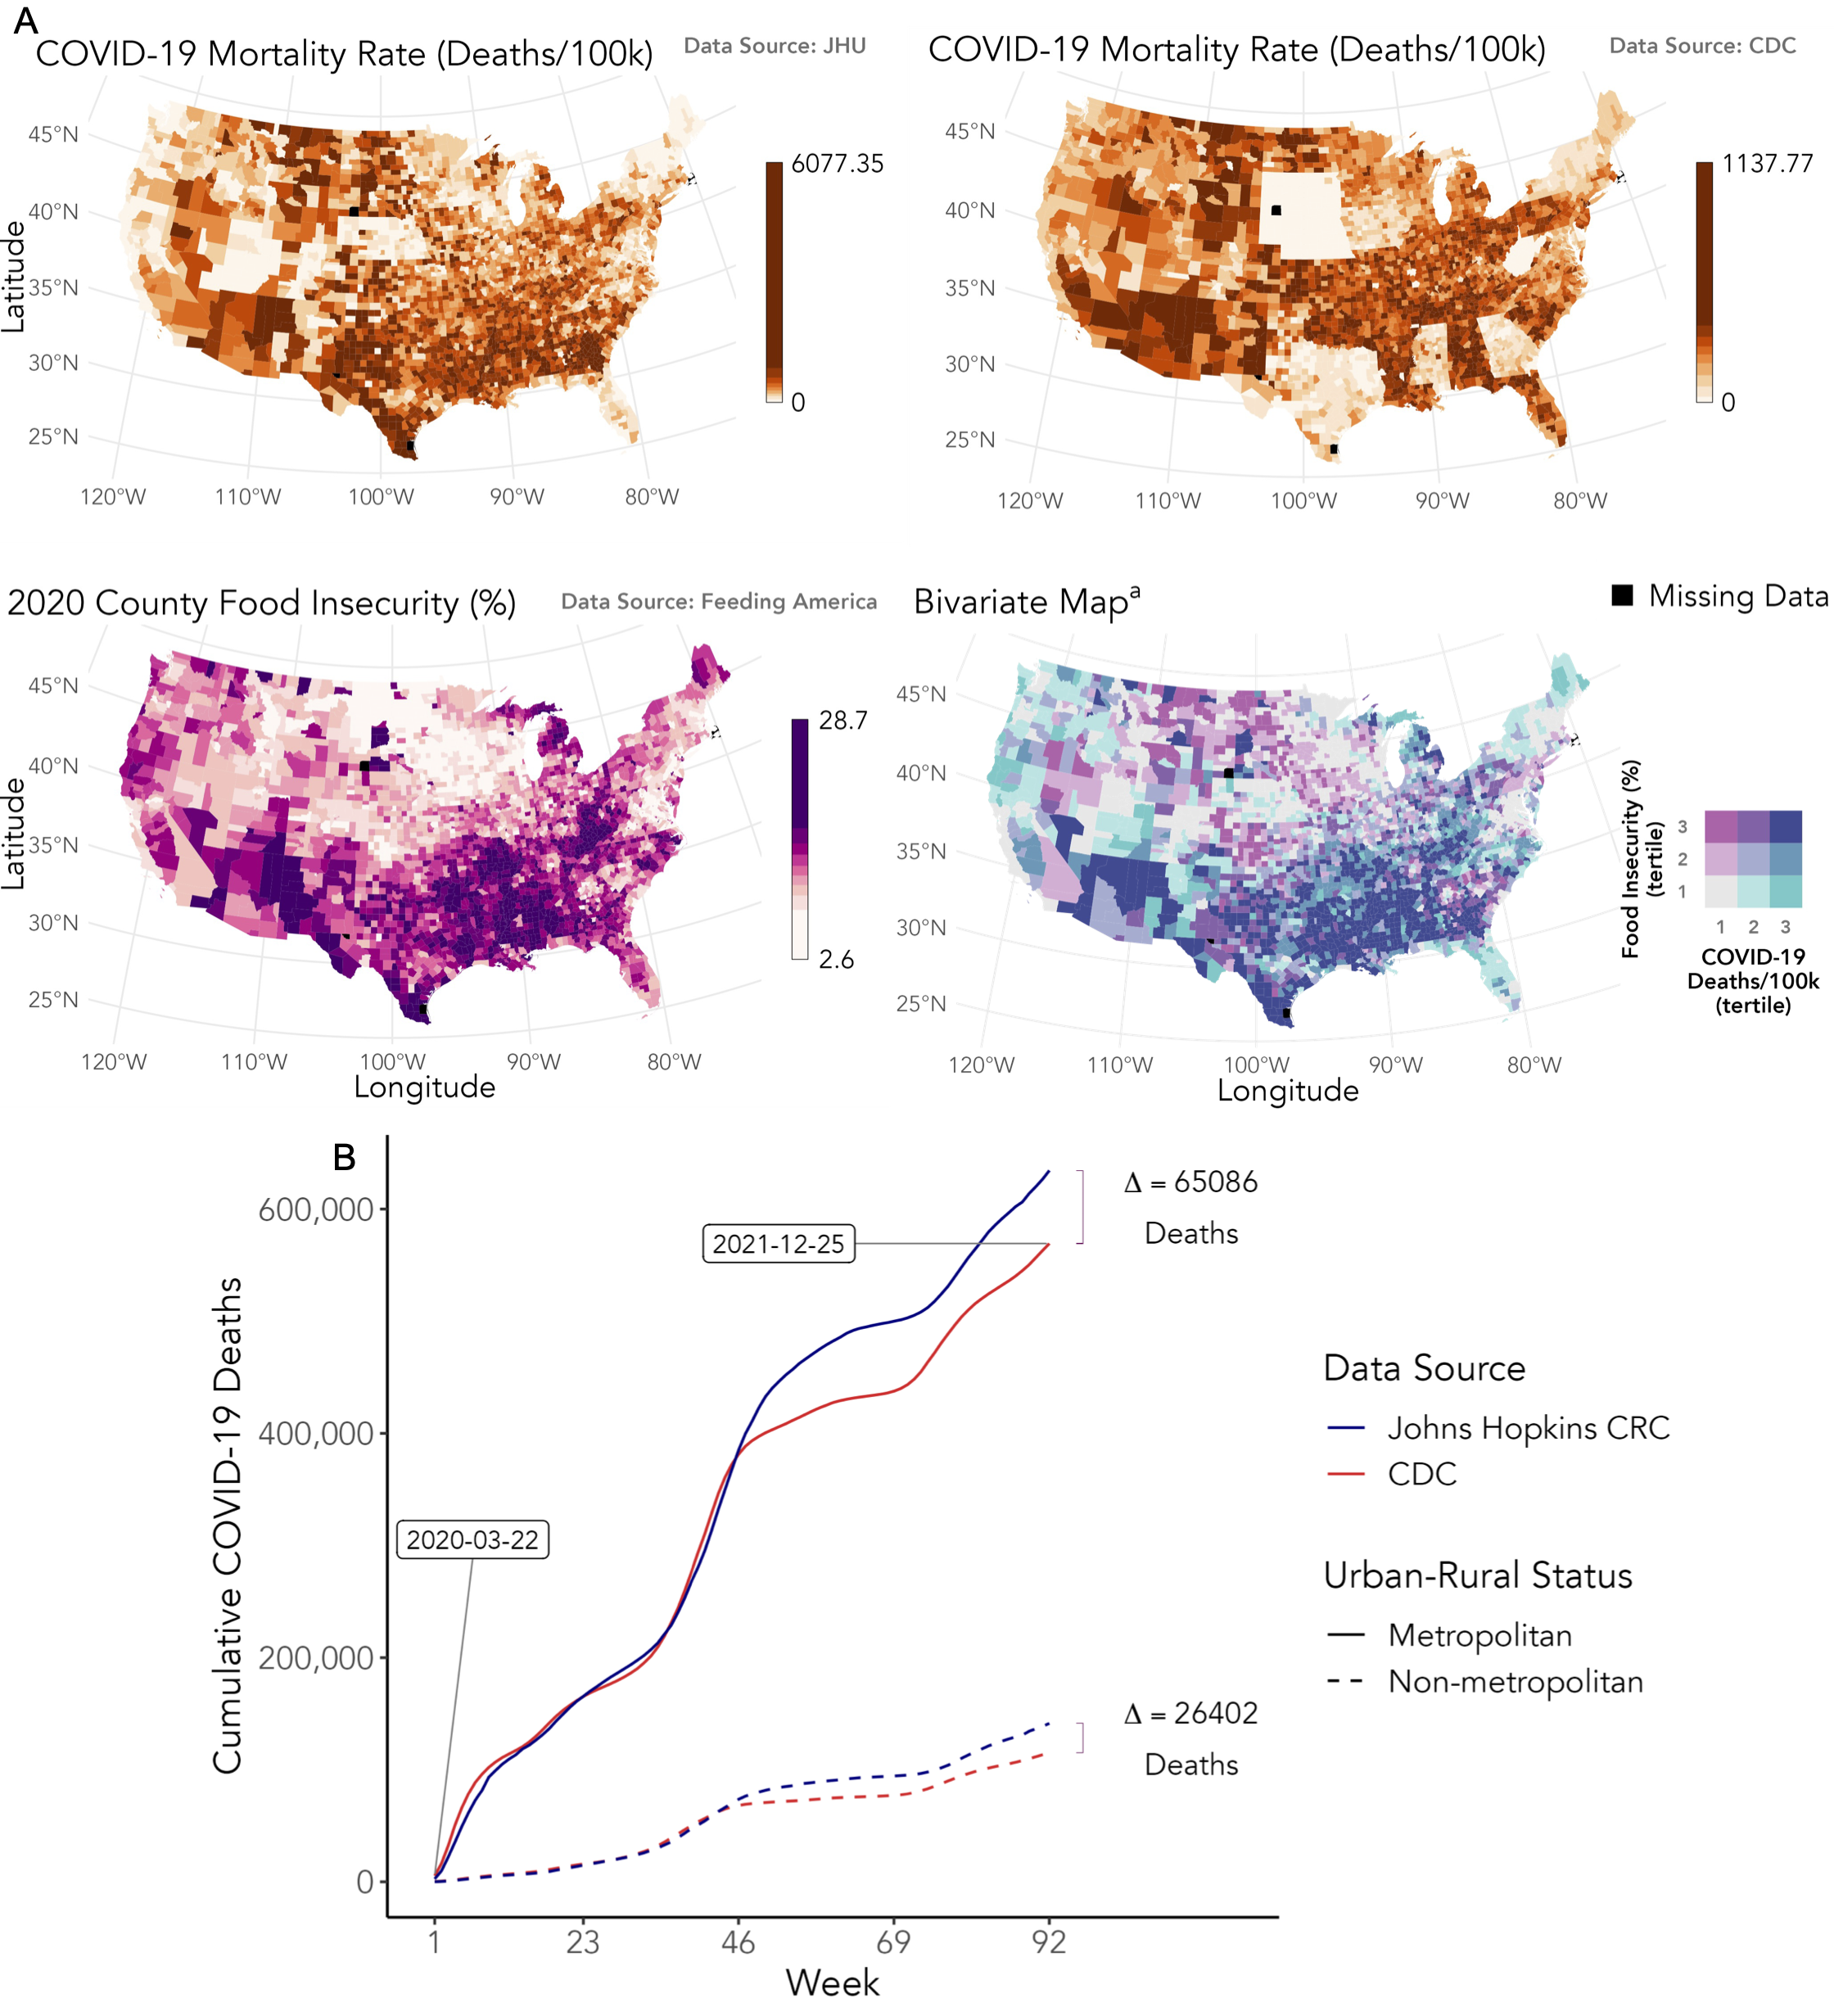
\includegraphics[scale=0.092]{images-logos/combo-chloro-time-series.png}\\
		
		
	\end{minipage}% the '%' is important for putting the mini pages side by side and not stacked
	\hspace{1.65 cm}
	\begin{minipage}{.30\textwidth}
			\vspace{-0.3 cm}
		\raggedright
	\tiny{\textbf{Figure 1}. \textit{Panel A}: Spatial distributions of the age-standardized dependent variables (from both the Johns Hopkins University Coronavirus Resource Center (JHU) and Centers for Disease Control and Prevention (CDC) data sources) and independent variable (food insecurity prevalence from Feeding America’s Map the Meal Gap). \\ 
		
\vspace{0.21cm}

		\textit{Panel B}: A time series depiction of the cumulative crude (not age- standardized) COVID-19 mortality counts, within the analytic time window, from both sources (mapped to the line colors) and further stratified on urban-rural status (mapped to the line-type). The starting and end dates plotted are based on the beginning and end dates of the first and last MMWR week for the analytic time window.}
		
	\end{minipage}
\end{frame}    

%% JHU results %%
 	\setbeamertemplate{logo}{} % remove logo on next slide
 \subsection{Spatial Models w/ INLA (JHU Data)}
\begin{frame}
	
	
	
	\vspace*{-0.02 cm}
	\hspace*{-0.35 cm}
	\centering
	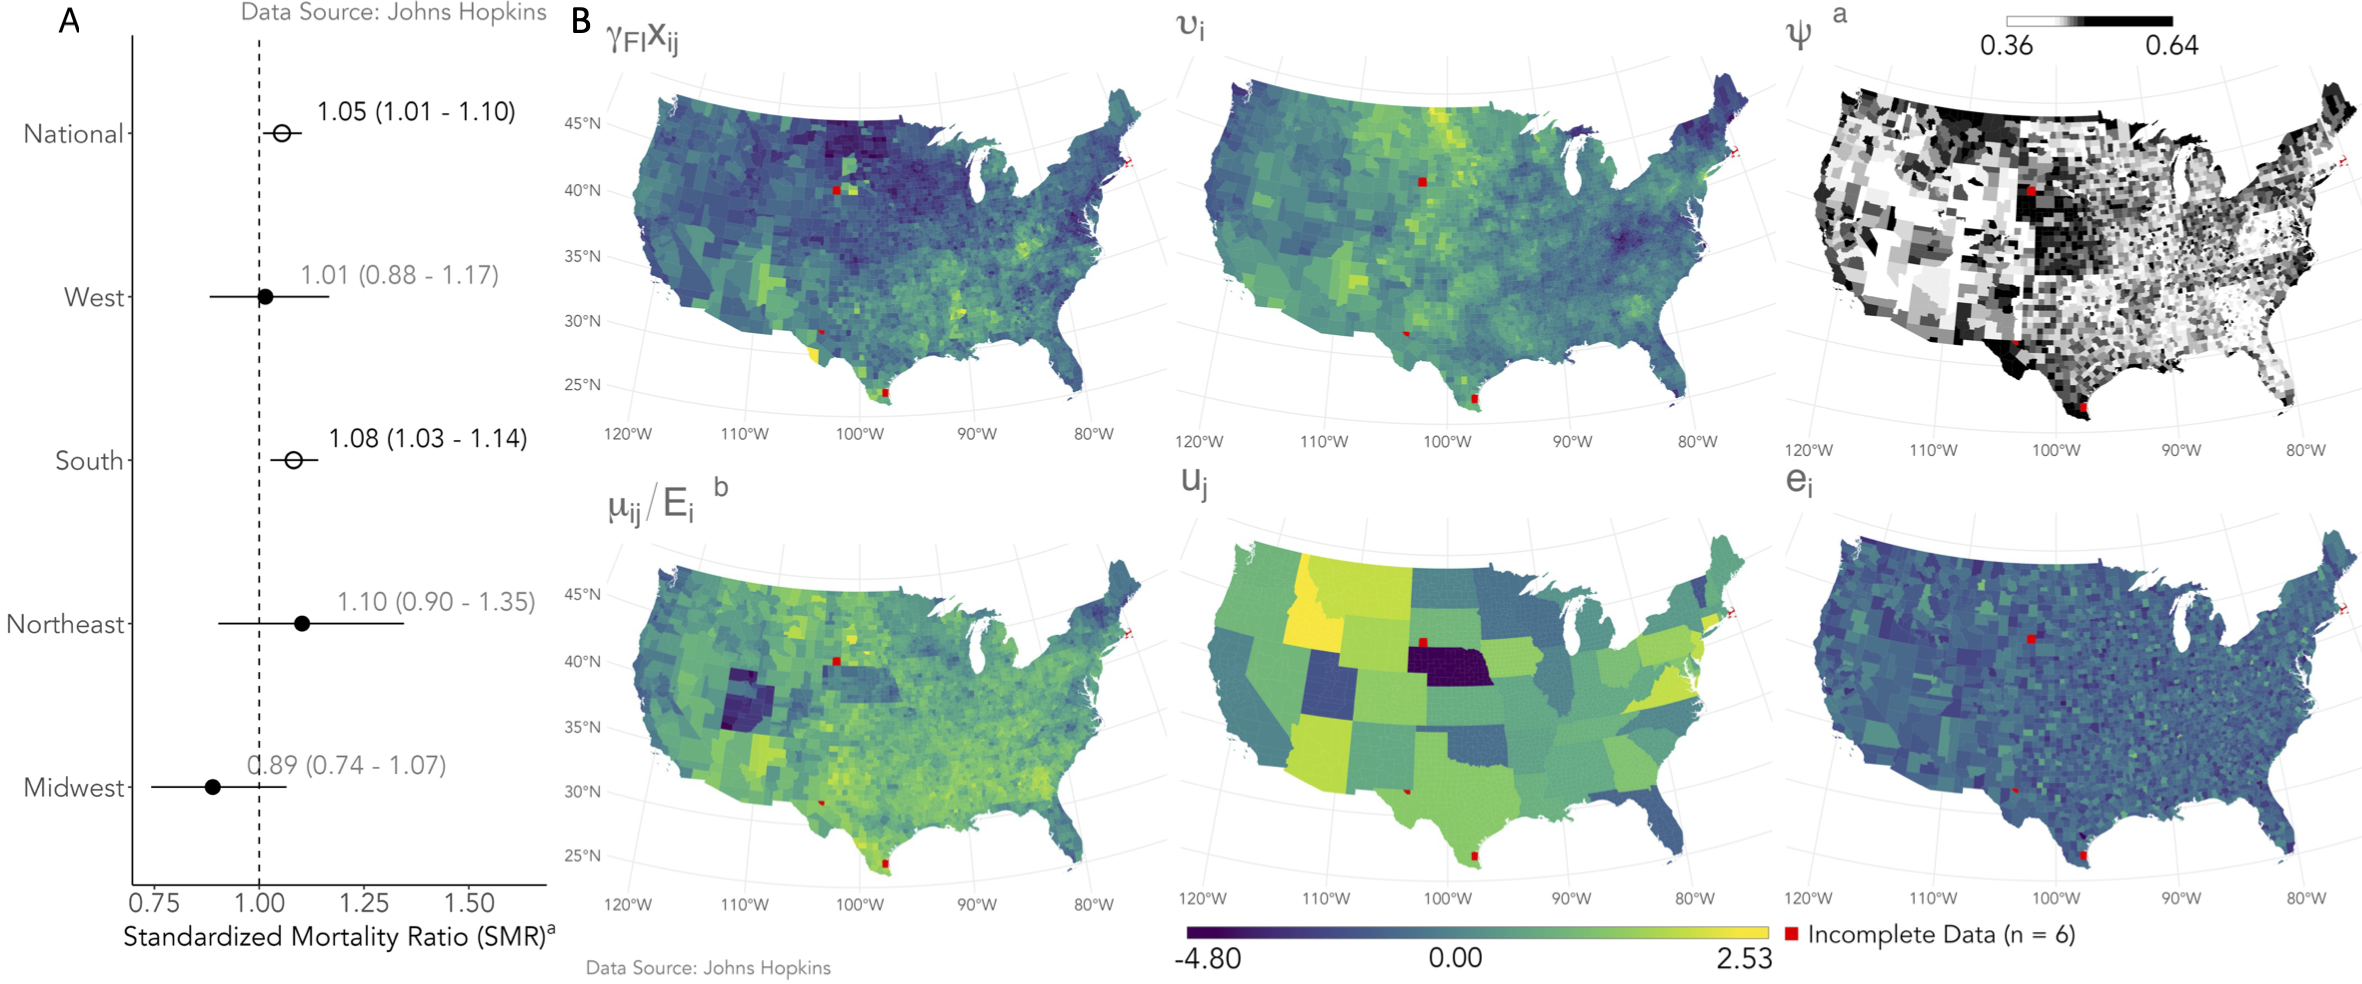
\includegraphics[scale=0.093]{images-logos/combo-forest-map-decomp-jhu.png}
	
	\raggedright
	\tiny{\textbf{Figure 2}. \textit{Panel A}: Means and their 95\% credible intervals (CrIs) for posterior distributions of the $exp(parameter)$ for the food insecurity (FI) fixed effect for the \textit{final model} (reflecting a standard deviation--4\%-- increase). A model was fit to the entire dataset (i.e., the National model--\textit{n} = 3102) and a stratified analysis was conducted per Census region. Open circles denote posterior means with 95\% CrIs whose bounds are completely above or below the reference value of 1 (dashed line). Results are shown for the analysis performed only on the age-standardized Johns Hopkins (JHU) COVID-19 mortality data. 
		
		\vspace{0.25cm}
		
		\textit{Panel B}: Map decomposition for the final model using national JHU data.\\
		$^a$ $\psi=\frac{SD(\upsilon)}{SD(\upsilon)+SD(u)+SD(e)}$;
		$^b$ The overall risk, or standardized mortality ratio (SMR) in the log scale, from the final model.\\
		The final model adjusted for county-level median age, health index score, and the standardized incidence ratio (SIR, state-level means of the health index score, the SIR, percent vaccinated, and the 2020 general election margin, percent female inhabitants and percent Hispanic inhabitants. Additional covariates in the final model were selected by forward selection with the Watanabe-Aikake Information Criterion (WAIC).}
	
	
\end{frame}

 \begin{frame}
\vspace*{-0.1cm}
			\begin{figure}
				\centering
				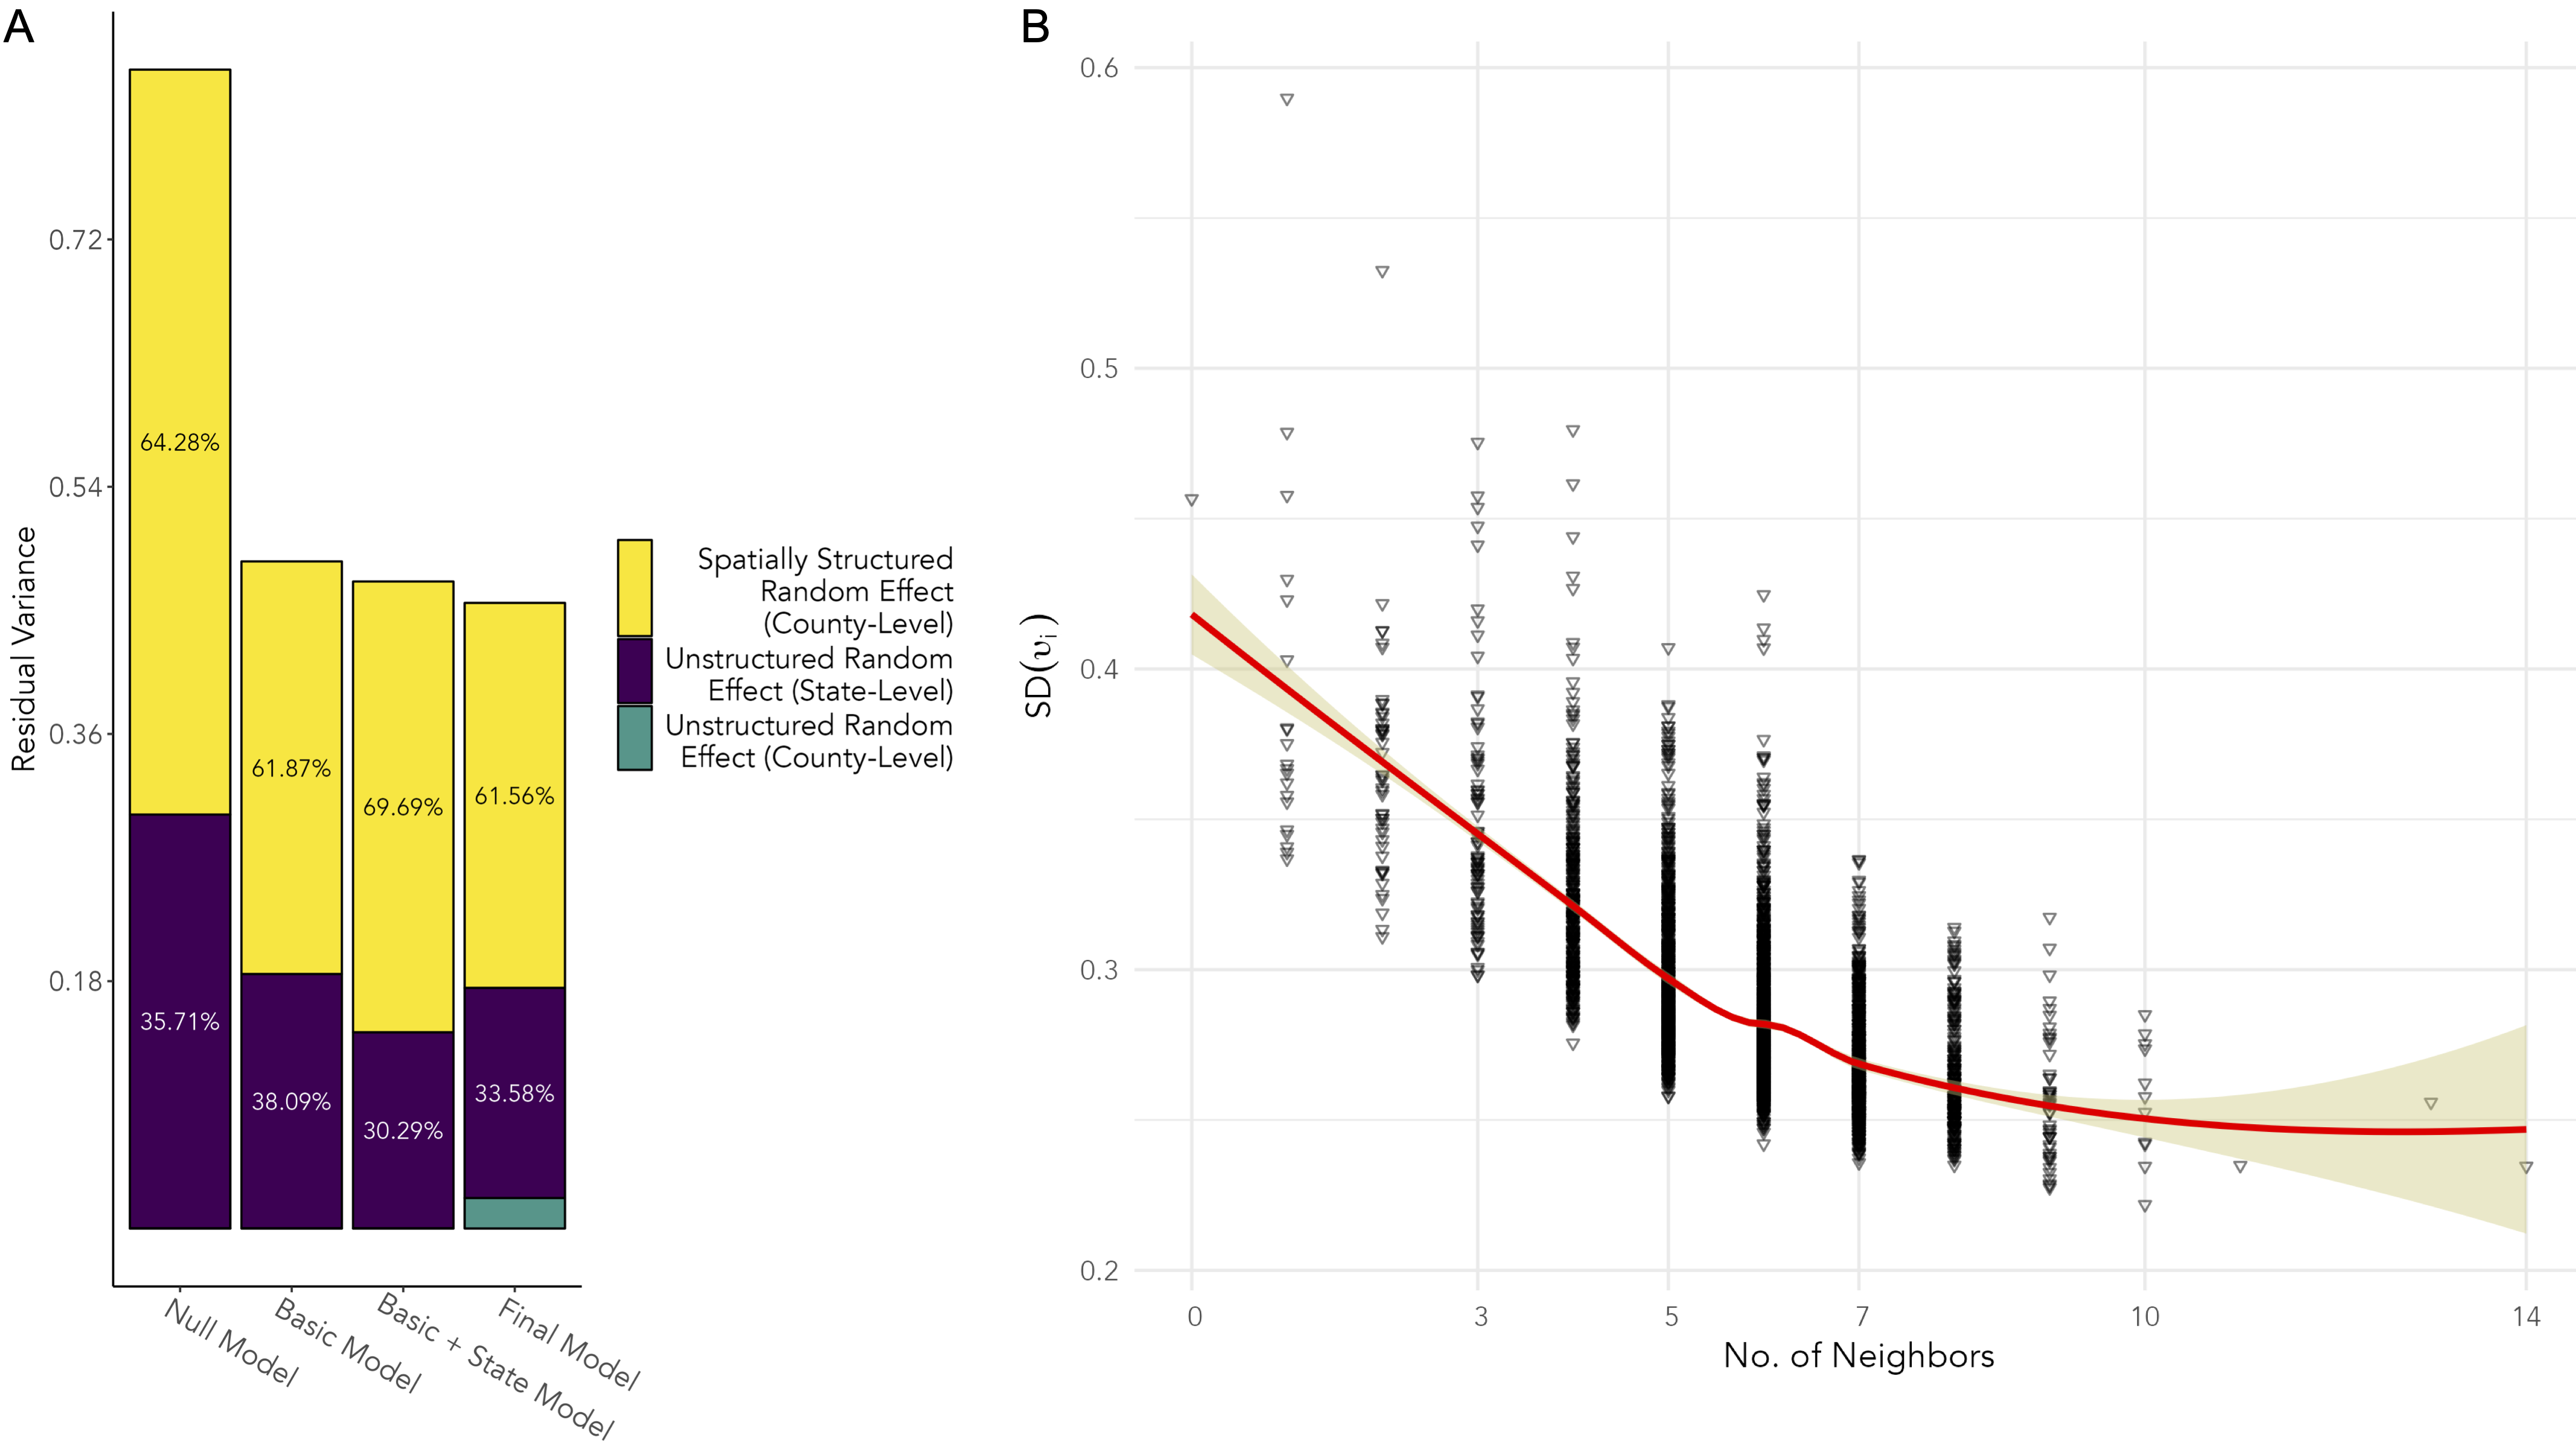
\includegraphics[scale=0.082]{images-logos/combo-res-var-nbs-jhu.png}
				
			\end{figure}      
			\vspace{-0.17cm}
			\tiny{\textbf{Figure 3}. \textit{Panel A}: Residual variance, computed as the sum of the variances of the random effects, across all models using national JHU data.\\  \textit{Panel B}: Standard deviation of the spatially structured random effect (in the final model using national JHU data) mapped to the number of neighbors. The LOESS smoother is shown.}



\end{frame}


 	\setbeamertemplate{logo}{} % remove logo on next slide
\subsection{Spatial Models w/ INLA (CDC Data)}
\begin{frame}
	
	
	
	\vspace*{-0.02 cm}
	\hspace*{-0.45 cm}
	\centering
	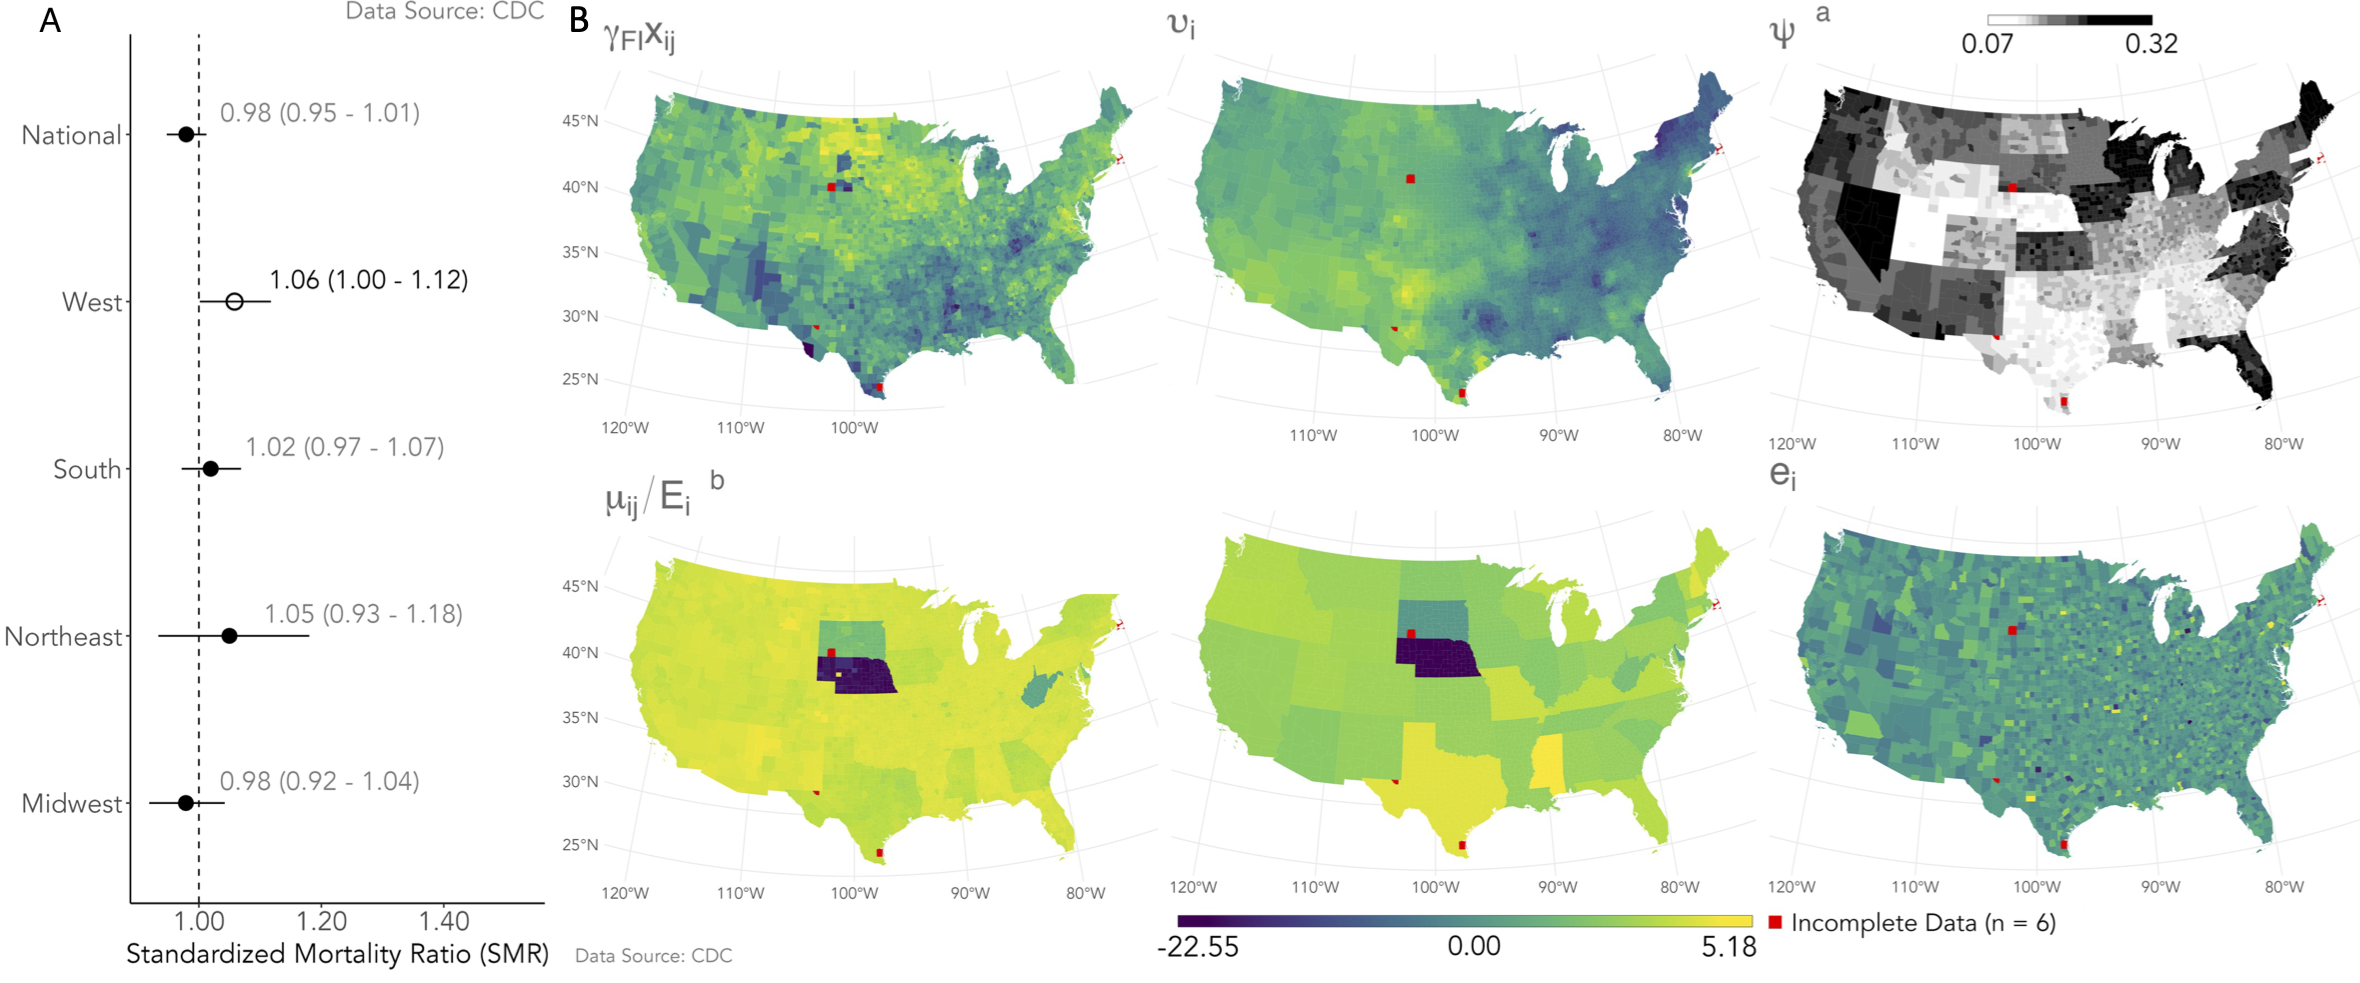
\includegraphics[scale=0.122]{images-logos/combo-forest-map-decomp-cdc.png}
	
	\raggedright
	\tiny{\textbf{Figure 2}. \textit{Panel A}: Means and their 95\% credible intervals (CrIs) for posterior distributions of the $exp(parameter)$ for the food insecurity (FI) fixed effect for the \textit{final model} (reflecting a standard deviation--4\%-- increase). A model was fit to the entire dataset (i.e., the National model) and a stratified analysis was conducted per Census region. Open circles denote posterior means with 95\% CrIs whose bounds are completely above or below the reference value of 1 (dashed line). Results are shown for the analysis performed only on the age-standardized CDC COVID-19 mortality data. 
		
		\vspace{0.25cm}
		
		\textit{Panel B}: Map decomposition for the final model using national CDC data.\\
		$^a$ $\psi=\frac{SD(\upsilon)}{SD(\upsilon)+SD(u)+SD(e)}$;
		$^b$ The overall risk, or standardized mortality ratio (SMR) in the log scale, from the final model.\\
		The final model adjusted for county-level median age, health index score, and the standardized incidence ratio (SIR, state-level means of the health index score, the SIR, percent vaccinated, and the 2020 general election margin, percent non-Hispanic White inhabitants. Additional covariates in the final model were selected by forward selection with the Watanabe-Aikake Information Criterion (WAIC).}
	
	
\end{frame}


\subsection{State Sensitivity Analysis: Spatial Models w/ INLA (CDC Data)}
\begin{frame}
	
	
	
	\vspace*{-0.02 cm}
	\hspace*{-0.45 cm}
	\centering
	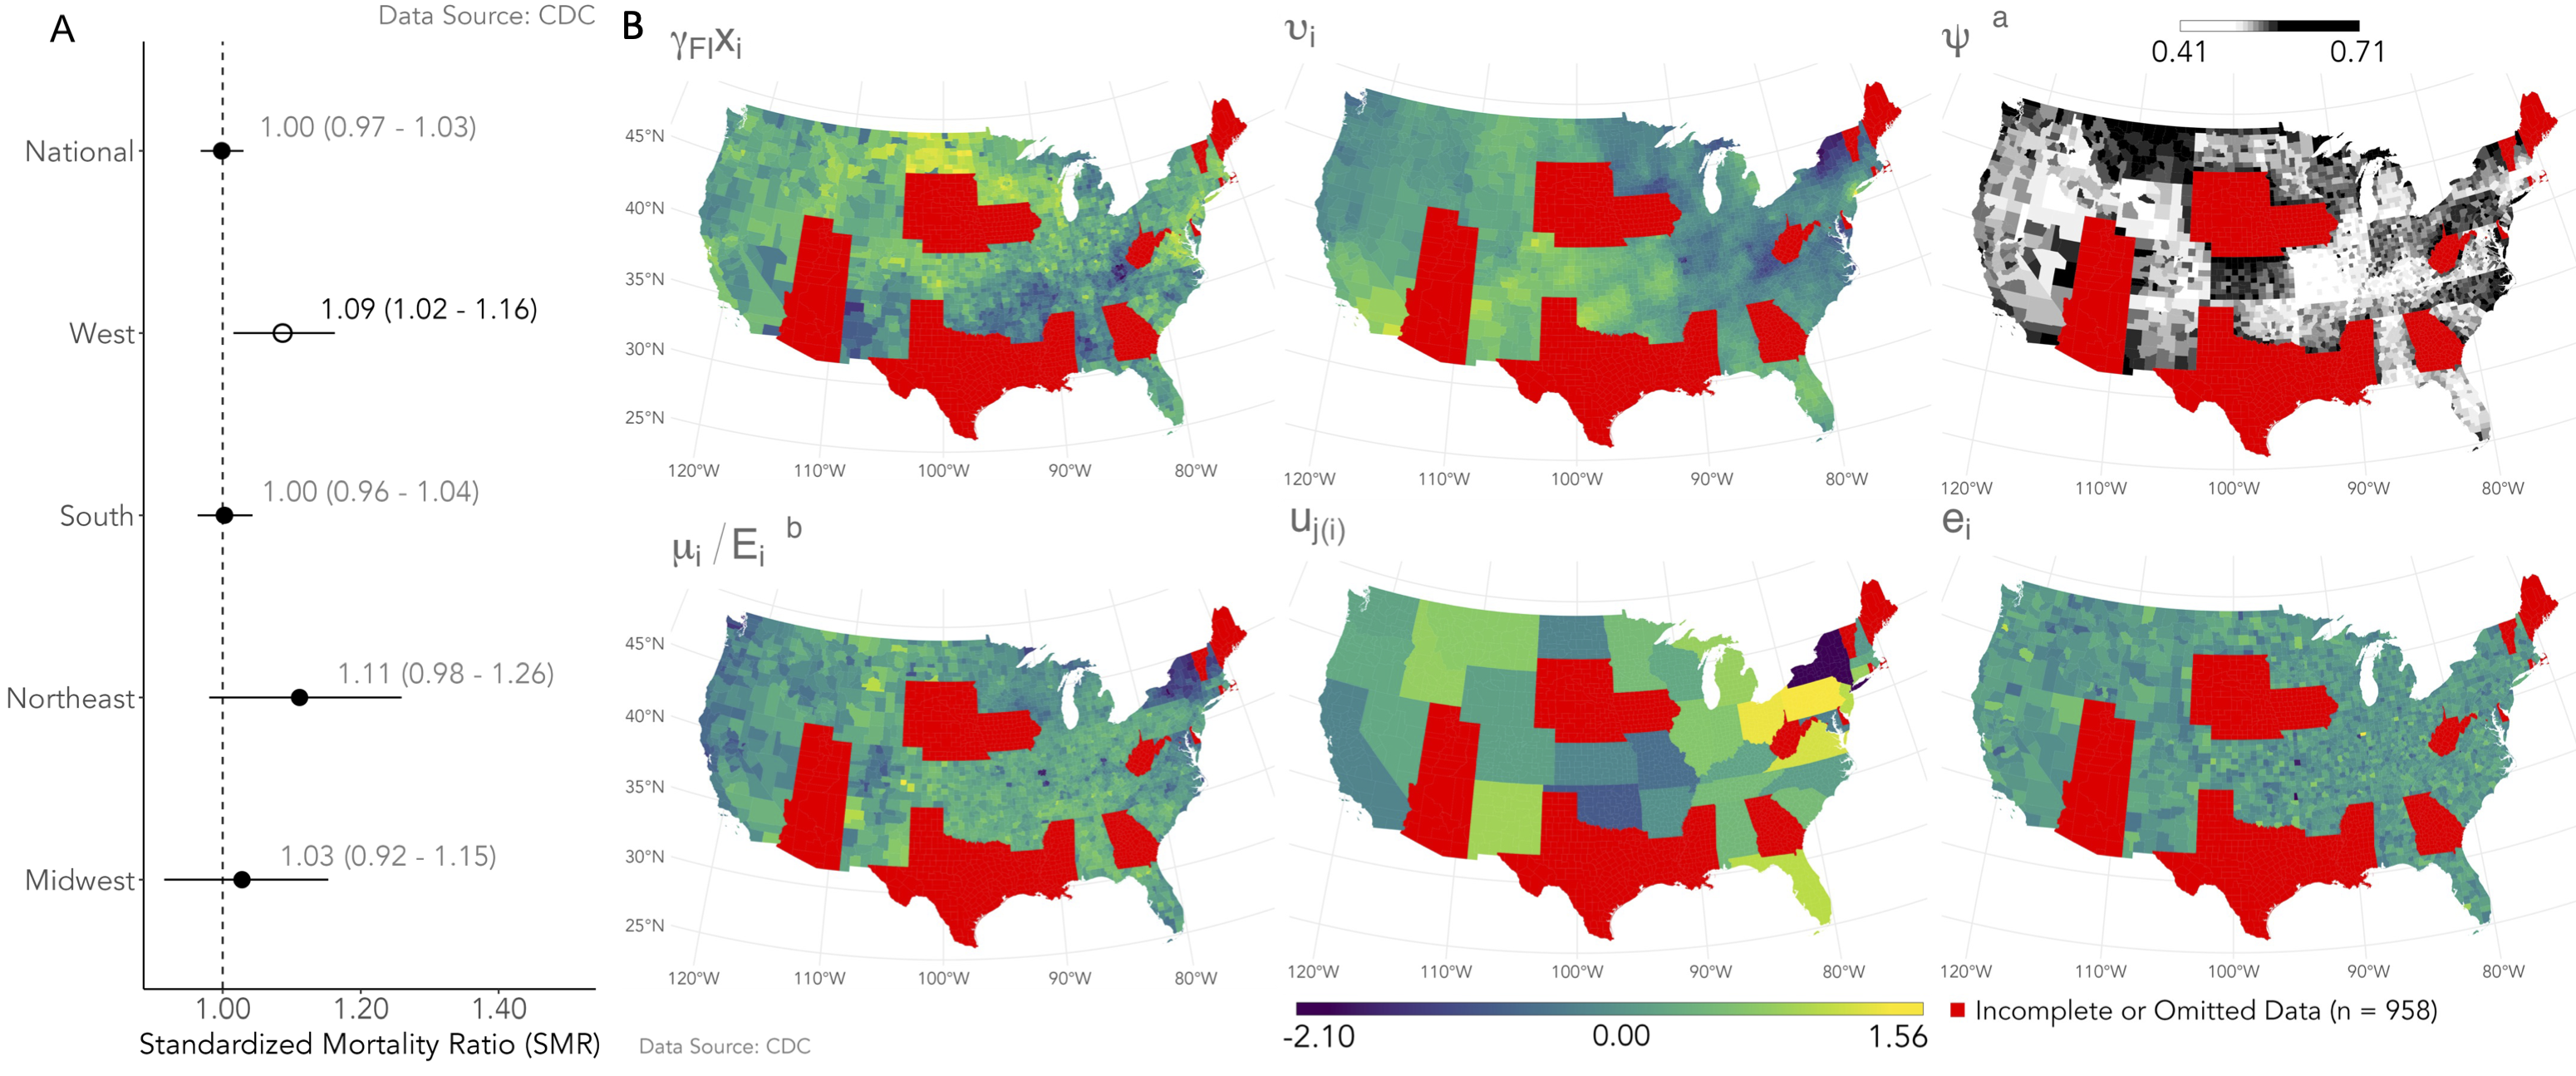
\includegraphics[scale=0.117]{images-logos/sensitivity-combo-forest-map-decomp-cdc.png}
	
	\raggedright
	\tiny{\textbf{Figure S5}. \textit{Panel A}: Means and their 95\% credible intervals (CrIs) for posterior distributions of the $exp(parameter)$ for the food insecurity (FI) fixed effect for the \textit{final model} (reflecting a standard deviation--4\%-- increase). A model was fit to the entire dataset (i.e., the National model) and a stratified analysis was conducted per Census region. Open circles denote posterior means with 95\% CrIs whose bounds are completely above or below the reference value of 1 (dashed line). Results are shown for the analysis performed only on the age-standardized CDC COVID-19 mortality data. 
		
		\vspace{0.25cm}
		
		\textit{Panel B}: Map decomposition for the final model using national CDC data.\\
		$^a$ $\psi=\frac{SD(\upsilon)}{SD(\upsilon)+SD(u)+SD(e)}$;
		$^b$ The overall risk, or standardized mortality ratio (SMR) in the log scale, from the final model.\\
		The final model adjusted for county-level median age, health index score, and the standardized incidence ratio (SIR, state-level means of the health index score, the SIR, percent vaccinated, and the 2020 general election margin, percent non-Hispanic White inhabitants. Additional covariates in the final model were selected by forward selection with the Watanabe-Aikake Information Criterion (WAIC).}
	
	
\end{frame}
	


\begin{frame}
		
\centering
		\vspace*{-0.19 cm}

		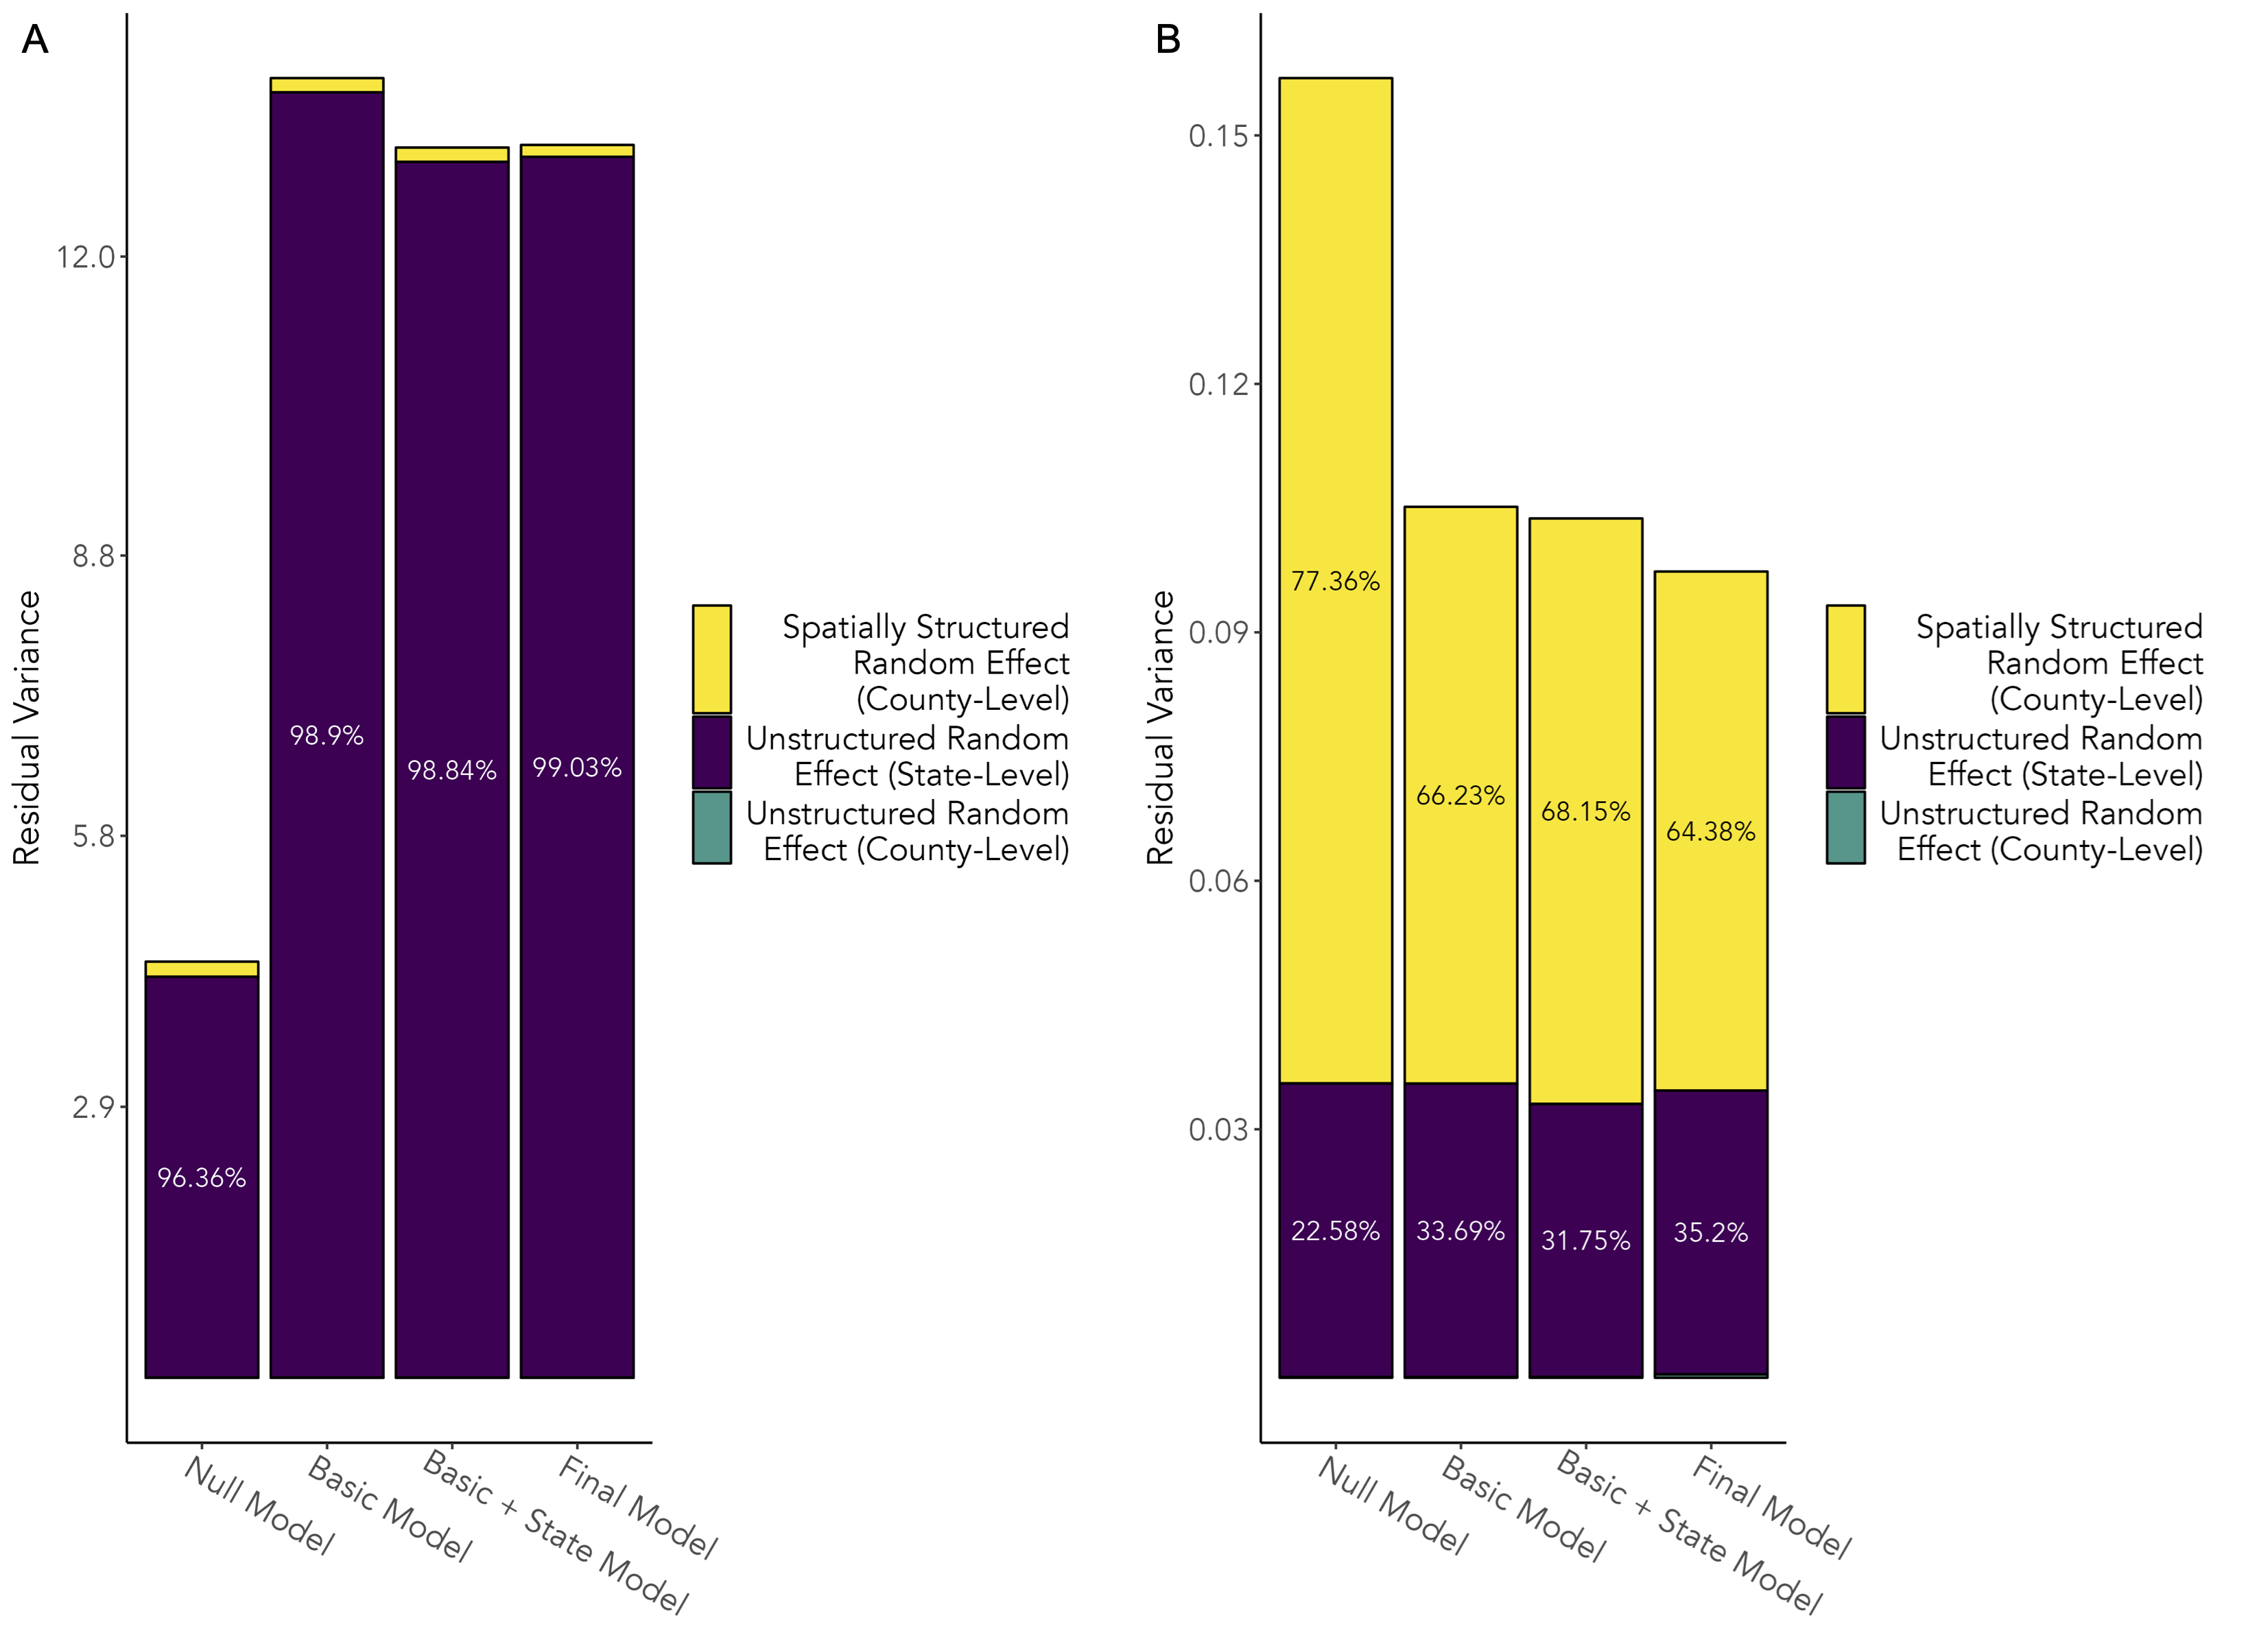
\includegraphics[scale=0.082]{images-logos/compare-cdc-res-var.png}
		
	
		
		\tiny{\textit{Panel A}: Total residual variance and relative composition from the main analysis using the CDC data (\textit{final model}).\\
			\textit{Panel B}: Total residual variance and relative composition from the state sensitivity analysis using the CDC data (\textit{final model}).}
			
\end{frame}

% conclusions
\section{Conclusion}
\subsection{Conclusions}
\begin{frame}
	\frametitle{Conclusions}
	\textbf{Conclusions and Strengths}:
	\begin{itemize}
		\item \textit{County-level food insecurity was positively associated with COVID-19 mortality}
		\begin{itemize}
			\scriptsize{
				\item Spatial autocorrelation
				\item Multivariable adjustment, age-standardization
				\item Regional specificity
				\item Robustness
			}
		\end{itemize}
		\item \textit{Gaps in COVID-19 mortality data?}
		\begin{itemize}
			\scriptsize{
				\item CDC vs. JHU
			}
		\end{itemize}
	\end{itemize}
	
	\textbf{Limitations}:
	\begin{itemize}
		\item Unmeasured confounding, causality
		\item Spatial resolution
		\item Aggregate data; ecological fallacy
	\end{itemize}
	
\end{frame}


  % acknowledgements
  \subsection{Acknowledgements}
\begin{frame}
	\frametitle{Acknowledgements}
	\vspace*{-0.3cm}
	\begin{multicols}{2} % split this into multiple columns
		
		\raggedright
	
		
		\textbf{Collaborators}
		
		\scriptsize{
			\begin{itemize}
				\item Rebecca L. Smith (\textit{Dept of. Pathobiology, Univ. of Illinois Urbana-Champaign (UIUC)})
				\item Mauricio Campos (\textit{Dept. of Statistics, UIUC})
				\item Sara L. McLafferty (\textit{Dept. of Geography and Geographic Information Science, UIUC})
				\item May A. Beydoun (\textit{LEPS, NIH/NIA})
				\item Anna E. Arthur (\textit{Dept. of Nutrition and Dietetics, Univ. of Kansas Medical Center})
				\item Francesca Gany (\textit{Memorial Sloan Kettering Cancer Center})
			
			\end{itemize}
		}
		
		% add github repo link
			\vspace{0.4cm}
			
			\scriptsize{
			\textbf{GitHub Repository (R Code and Data)}

\textcolor{blue}{\href{https://github.com/cmainov/covid-fi-mortality-mirror}{github.com/cmainov/covid-fi-mortality-mirror}}
		
		}
		% both below are needed for the column break
		\vfill\null
		\columnbreak
		
		
		\scriptsize{
			\textbf{2023 HPRS Writing Retreat}
			\begin{itemize}
				\item Jeronimo Cortina (\textit{Univ. of Houston})
				\item Alex Maxim (\textit{Georgia Tech Univ.})
				\item Nayla Bezares (\textit{Tufts Univ.})
			\end{itemize}
		}
		
		\vspace{0.1cm}
		
		\textbf{Funding}
		\vspace{0.2cm}
		\scriptsize{
			\begin{itemize}
				\item \textit{Robert Wood Johnson Foundation (RWJF) Health Policy Research Scholars (HPRS)}
			\end{itemize}
		}
		
		\textbf{Data}
		\vspace{0.1cm}
		\scriptsize{
			\begin{itemize}
				\item \textit{CDC}
				\item \textit{JHU CRC}
				\item \textit{2023 County Health Rankings--RWJF and Univ. of Wisconsin}
			\end{itemize}
		}
		\vspace{0.4cm}
		
		% shift github logo and link to the right
	 \hspace*{2.80cm}	\faGithub \hspace{0.05cm} \textcolor{blue}{\href{https://github.com/cmainov}{github.com/cmainov}}
	\end{multicols}
	
\end{frame}

\end{document}


%% End of Document %%
%%%%%%%%%%%%%%%%%%%%%%%%%%%%%%%%%%%%%%%%%%%%%%%%%%
